\documentclass[11pt]{article}
\usepackage{classTools}

\begin{document}

% To include a problems set header, use the psHeader command
\psHeader{4}{Wed Oct. 9, 2024 (11:59pm)}

\textbf{Your name: }Emily Kang

\textbf{Collaborators: }

\textbf{No. of late days used on previous psets: } 0 

\textbf{No. of late days used after including this pset: } 0 

\begin{enumerate}
    \item (Randomized Algorithms in Practice)  
    \begin{enumerate}
        \item Implement Randomized QuickSelect, filling in the template we have given you in the Github repository. \\
        \textit{Solution.} In python file.
        \item 
        In the repository, we have given you datasets $x_n$ of key-value pairs of varying sizes to experiment with: dataset $x_n$ is of size $n$.  For each dataset $x_n$ and any given number $k$, we will consider how to efficiently answer the $k$ selection queries
        $\select(x_n,0)$, $\select(x_n,[n/k])$, $\select(x_n,[2n/k])$, $\ldots$, $\select(x_n,[(k-1)n/k])$ on $x_n$, where $[\cdot]$ denotes rounding to the nearest integer. For example, if $k=4$, then we release the minimum, the 25th percentile, and the 75th percentile of the dataset.  You will compare the following two approaches to answering the queries:
        
        \begin{enumerate}
            \item Running (randomized) \QuickSelect{} $k$ times.
            \item Running \MergeSort{} (provided in the repository) once and using the sorted array to answer the $k$ queries.
        \end{enumerate}
        Specifically, you will compare the {\em distribution} of runtimes of the two approaches for a given pair $(n,k)$ by running each approach many times and creating density plots of the runtimes.  The runtimes will vary because \QuickSelect{}  is randomized, and because of variance in the execution environment (e.g. other processes that are running on your computer during each execution). \vspace{1.5mm} 
        
        We have provided you with the code for plotting. Before plotting, you will need to implement \MergeSortSelect{}, which extends \MergeSort{} to answer $k$ queries. Your goal is to use these experiments and the resulting density plots to propose a value for $k$, denoted $k^*(n)$, at which you should switch over from \QuickSelect{} to \MergeSortSelect{} for each given value of $n$ (you can choose any reasonable statistical feature to propose $k^*(n)$, such as the peak runtime of the distribution or the mean runtime, etc). Do this by experimenting with the parameters for $k$ (code is included to generate the appropriate queries once the $k$'s are provided) and generate a plot for each experiment.  Explain the rationale behind your choices, and submit a few density plots for each value of $n$ to support your reasoning.  (There is not one right answer, and it may depend on your particular implementation of \QuickSelect{}.)

        \textit{Solution:}
        \begin{figure}[H]
            \centering
            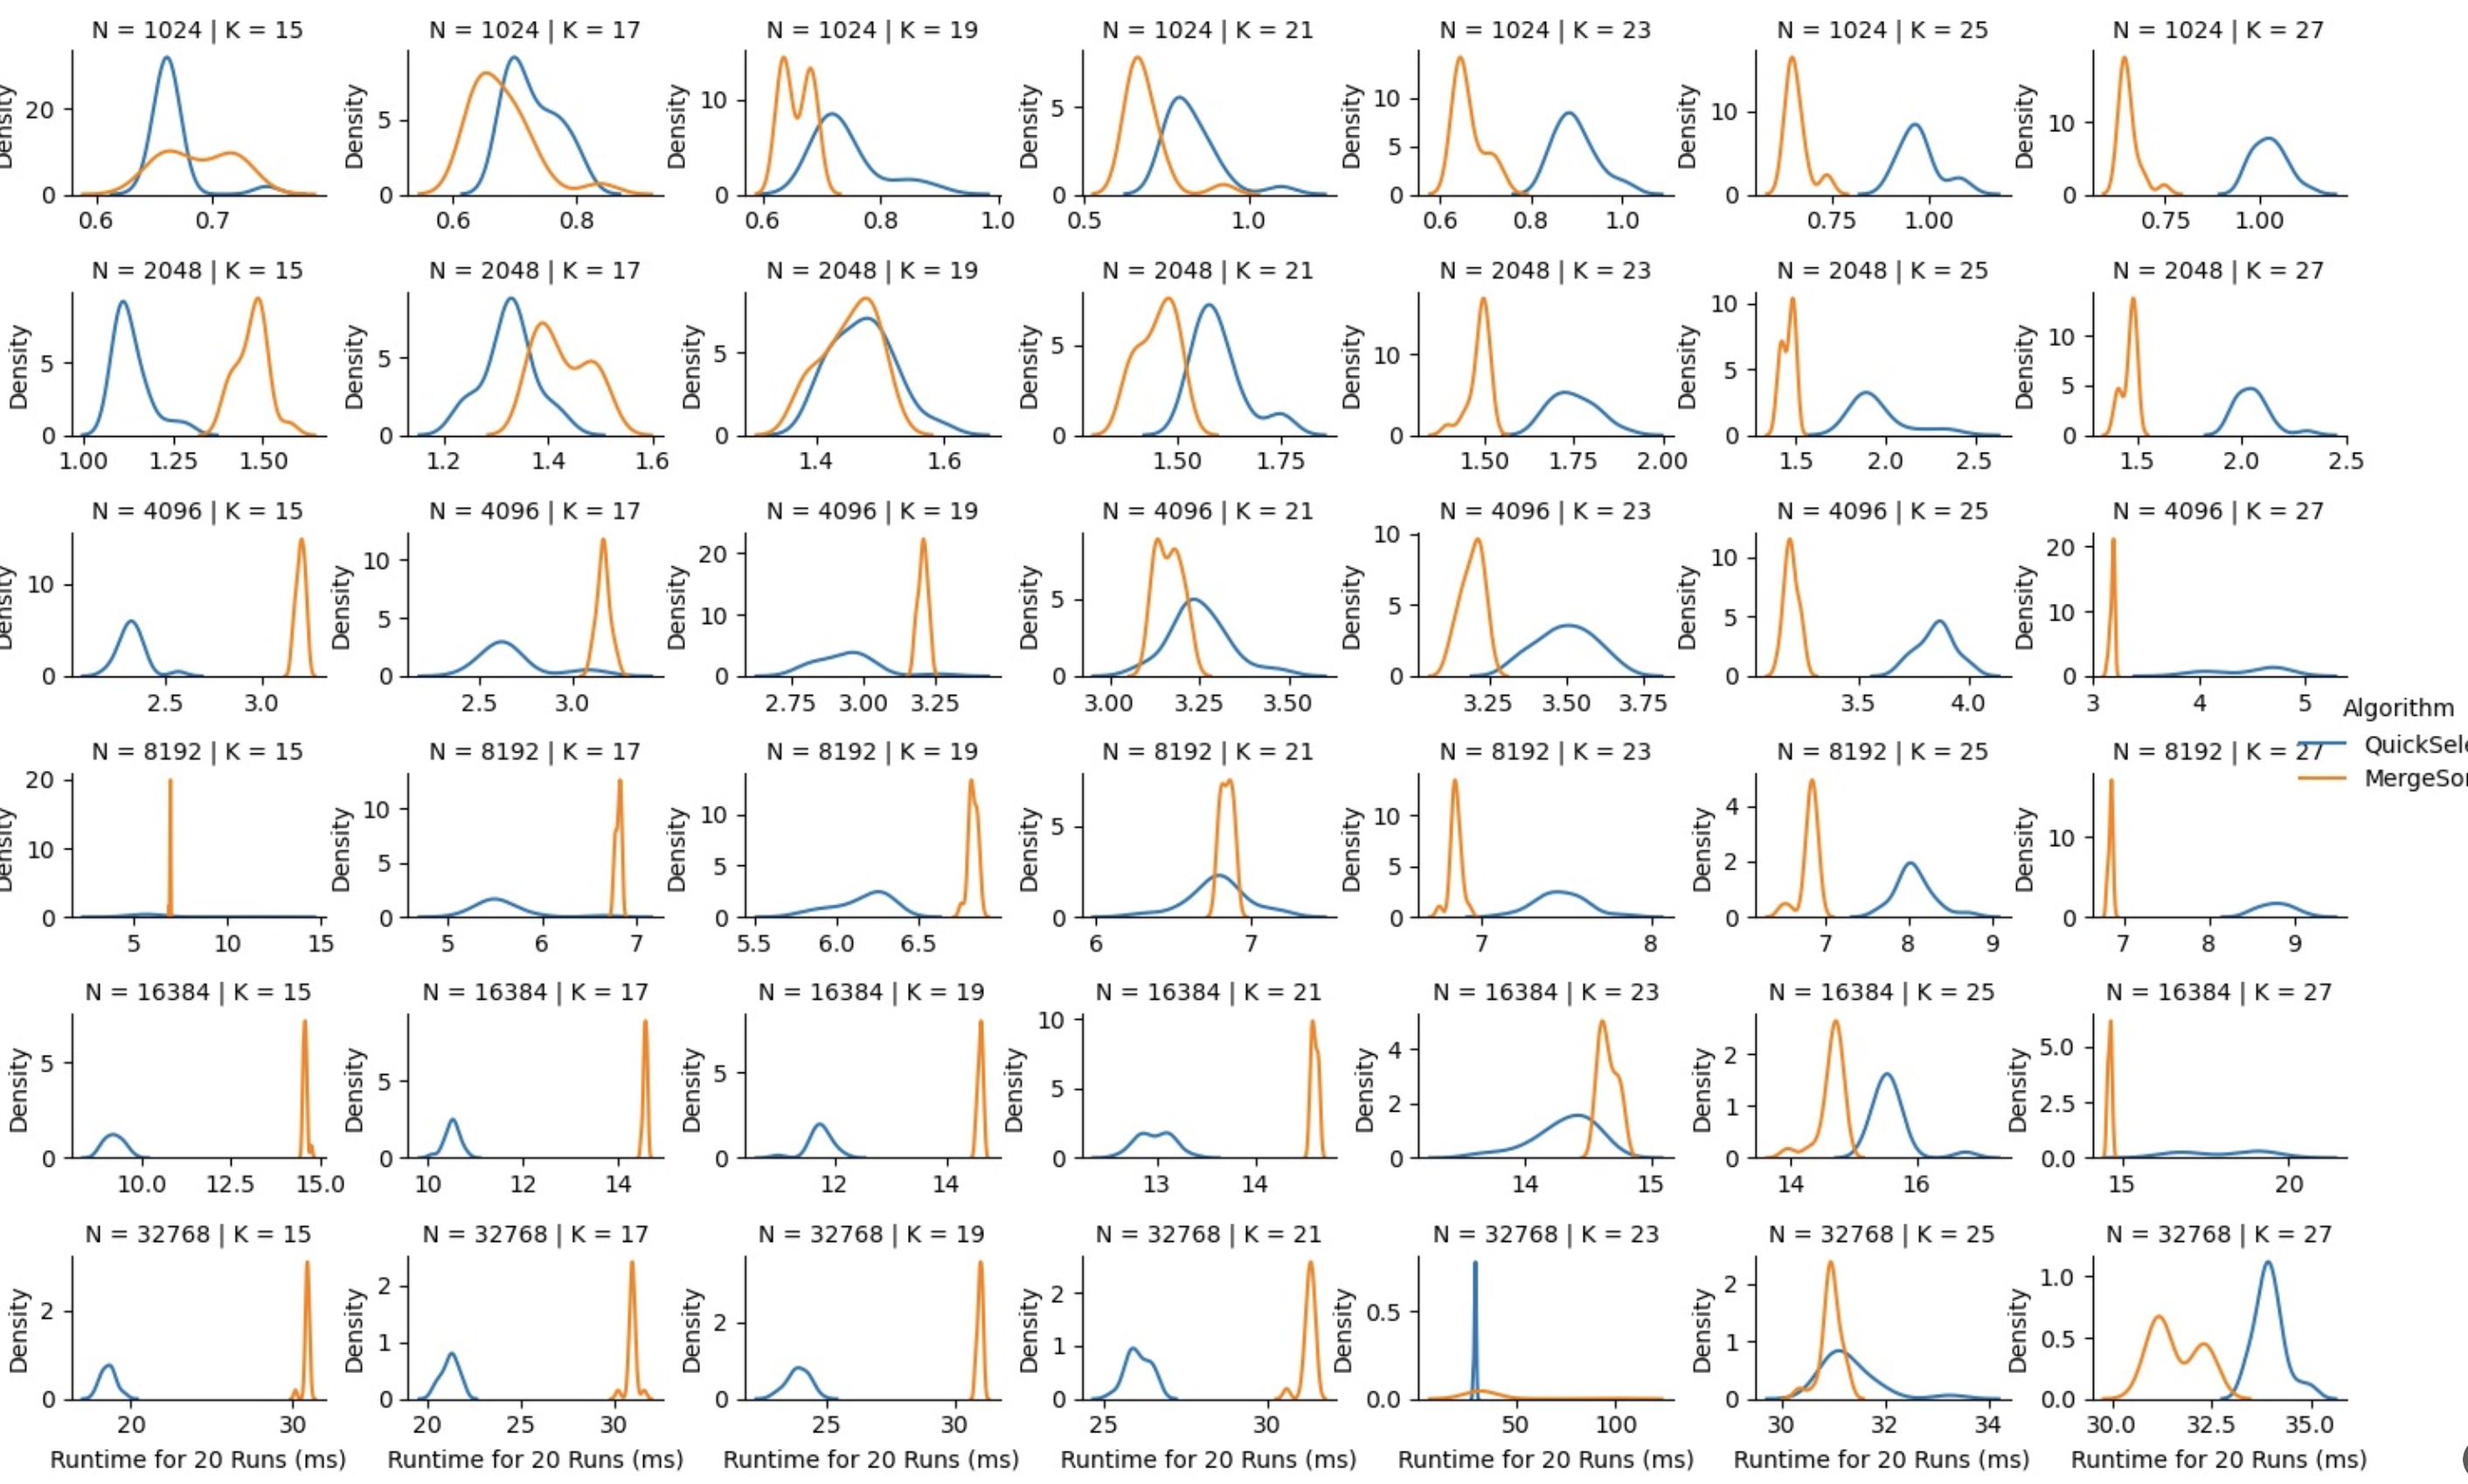
\includegraphics[width=\textwidth]{graph.png}
            \caption{MergeSort and QuickSelect on varying dataset sizes.}
            \label{fig:graph}
        \end{figure}
        
        \begin{enumerate}
            \item For \( N = 2^{10} \), \( k^*(N) = 17 \)
            \item For \( N = 2^{11} \), \( k^*(N) = 19 \)
            \item For \( N = 2^{12} \), \( k^*(N) = 21 \)
            \item For \( N = 2^{13} \), \( k^*(N) = 21 \)
            \item For \( N = 2^{14} \), \( k^*(N) = 23 \)
            \item For \( N = 2^{15} \), \( k^*(N) = 25 \)
        \end{enumerate}
        
        We can see that based on the trials, we have the above values for $k^*(N)$. The rationale behind each of these choices for $k^*(N)$ is that can observe that $k^*$ seems to increase linearly as $n$ increases exponentially. We do, in fact see that when we roughly eyeball the mean of the distributions, as we can see the value of $k$ for which the mean of QuickSelect overtakes the mean of MergeSort. Then, we can report each $k$ in relation to its corresponding $N$ value.
        
        \item Extrapolate to come up with a simple functional form for $k^*(n)$, e.g. something like $k^*(n)=3\sqrt{n}+6$ or $k^*(n)=10\log^2 n$. (Again there is not one right answer.)  Briefly discuss how your extrapolation aligns with theoretical values. That is, what kind of functional form for $k^*(n)$ (in asymptotic notation) would be predicted by  the asymptotic runtimes of \QuickSelect{} and \MergeSortSelect{} for answering $k$ selection queries on a dataset of size $n$? 
        
        \textit{Solution. }The asymptotic runtime to make $k$ queries of \QuickSelect{} is $O(kn)$ and the asymptotic runtime to make $k$ queries of \MergeSortSelect{} is $O(nlogn + k)$, as it takes constant time to query after sorting. Then, setting these runtimes equal to find $k$, we have
        $$ k^*(N) = \frac{n}{n-1} log(n).
        $$
        However, for large n, the fraction approaches $1$, and once we consider constant factors, we end up with
        $$ k^*(N) = a\cdot logn + b
        $$
        for some constants $a$ and $b$. Based off of our empirical results, this could be in the form 
        $$ \boxed{k^*(N) = 2log(n) - 3}.
        $$
        (For the base $2$ logarithm.)
        \item (*optional)  One way to improve \QuickSelect{} is to choose a pivot more carefully than by picking a uniformly random element from the array. A possible approach is to use the \textit{\textbf{median-of-3}} method: choose the pivot as the median of a set of 3 elements randomly selected from the array. Add \MedianQuickSelect{} to the experimental comparisons you performed above and interpret the results.  That is, in what way (if any) does \MedianQuickSelect{} offer benefits over \QuickSelect{}?        
        
    \end{enumerate}


    \item (Dictionaries and Hash Tables) 
    Consider the following computational problem:
    
\compprob{DuplicateSearch()}
{An array $(a_0,\ldots,a_{n-1})$ of natural numbers (each fitting in one word).}
{A duplicate element; that is, a number $a$ such that there exist $i \neq j$ such that $a_i = a_j = a$.}
\begin{enumerate}
    \item Show that DuplicateSearch can be solved by a Las Vegas algorithm with expected runtime $O(n)$ using a dictionary data structure.  (You should prove correctness and analyze runtime quoting the expected runtimes stated for the Dictionary data structure in Lecture 9, but you do not need to do a formal probability calculation using expectations.)  

    \textit{Solution. }A Las Vegas algorithm with expected runtime $O(n)$ that solves DuplicateSearch can be as follows:

    In the process of initializing a hash table, first check if the current element being inserted already exists, and if so, return the current element. In more detail, 
    \begin{enumerate}
        \item Preprocess: Initialize an array $A$ of size $m = \Theta (n)$. In adddition, choose a rantom hash function $h: [U] \rightarrow [m]$ from the universe $[U]$ to $[m]$.
        \item Search and Insert: Iterate through the input array. For each element $a_j$,
        \begin{enumerate}
            \item Search: Walk through the linked list at slot $A[h(a_j)]$ and exit and return the first element of the list that matches the natural number $a_j$
            \item Insert: Else, if $a_j$ was not found during Search, Insert $a_j$ by placing $a_j$ into the linked list (as the head) at slot $A[h(k)]$.
        \end{enumerate}
        \item After interating through every element of the input array, return $\perp$.
    \end{enumerate}

    \textbf{Proof of Correctness: } We will now prove the correctness of this algorithm. As a disclaimer, for simplicity of notation we will use $1$ indexing. The loop invariant is that as we iterate throught the input array, at then end of the $jth$ loop, all unique elements up until and including the $jth$ element will be included in our hash table $A$, and if the $j$th element is a duplicate we will immediately return it. This guarantees that we will catch some duplicate if it exists. 

    We will use proof by induction. For the base case, note that this is immediately true for the first element inserted into the hash table, as it must be unique. Now assume that the loop invarriant holds for the $j$th element of the input array. We will show that the loop invariant also holds for the $j+1$th element of the input array.

    At this point, there only exist $k$ unique elements in the hash table $A$, where $k \leq j$. If the $j+1$th element of the input array is not unique, an equivalent natural number will be found in $A$ through search, and we will return this element. Otherwise, the element is unique and will be inserted into $A$ through Insert. Therefore, the loop invariant holds.

    Thus we have shown by induction that the algorithm will return any duplicates if they exist, otherwise it will proceed to the end of the loop without returning anything, in which case it will return $\perp$.

    \textbf{Runtime: } The algorithm takes $O(n)$ time to initialize the array during preprocessing. Then, for each element of the input array, Search, Insert, etc. take constant time, so for all $n$ elements this would take $O(n)$ runtime. Therefore the total runtime is \boxed{O(n)}.
    \item DuplicateSearch can be solved by a deterministic algorithm in runtime $O(n\log n)$. Briefly describe this algorithm in 2-3 sentences (you do not need to write a pseudocode and do not need to provide a proof of correctness).

    \textit{Solution. } DuplicateSearch can be solved by an algorithm that makes a call to a sorting oracle such as MergeSort and then iterates through the sorted array, comparing adjacent elements and checking if they are equal. If they are, return one of these elements. Otherwise if we make it to the end of the array and have found no duplicates, return $\perp$. More formally, the call to MergeSort takes $O(nlogn)$ runtime, and when we iterate through the $n$ elements of the array, we can check for each element $a_j$ for $j$ in ${0, ..., n-2}$, whether or not it is equal to the $j+1$th element $a_{j+1}$. This has a runtime of $O(n)$. Therefore the final runtime is $O(nlogn) + O(n) = \boxed{O(nlogn)}$.
\end{enumerate}    
    

 \item (Choosing Algorithms and Data Structures)
     Suppose the US Census Bureau was going to develop a new database to keep track of the exact ages of the entire US population, and publish statistics on it.  The data it has on each person is an exact birthdate
    $\bday$ (year, month, and date) and a unique identifier $\id$ (e.g. social security number --- pretend that these are assigned at birth). 
    
    For each of the three scenarios below, 
    \begin{enumerate}
        \item Select the best algorithm or data structure for the Census Bureau to use from among the following: 
        \begin{itemize}
            \item sorting and storing the sorted dataset 
            \item storing in a binary search tree (balanced and possibly augmented)
            \item storing in a hash table
            \item running randomized QuickSelect. 
        \end{itemize}
        \item Explain how you would use the
        algorithm or data structure (including any necessary augmentations) to solve the stated problem, e.g. what would you take as keys and values, what updates and queries (in case you use a dynamic data structure) would you issue, and how you would read off the results to obtain the desired statistics. 
        \item State what the runtime would be as a function of all of the relevant parameters: the size $n$ of the US population being surveyed, the number $u$ of updates issued at the specified time intervals, and/or the number $s$ of statistics released at the specified time intervals.     (These parameters are not all freely varying in the parts below, e.g. $s$ may be a fixed constant or a function of $n$; state any such constraints in your answers.) 
    \end{enumerate}
    In each scenario, you should assume (unrealistically) that the described queries or statistics are the {\em only} way in which the data is going to be used, so there is no need to support anything else.
        
\begin{enumerate}
    \item (Reporting Age Rankings)
    Every ten years as part of the Decennial Census, the Bureau collects a fresh list of $(\id,\bday)$ pairs from the entire US population.
    (It does not reuse data from the previous Decennial Census, so everyone is re-surveyed.)
    In order to incentivize participation, the Bureau promises to tell every respondent their age-ranking in the population after the survey is done (e.g. ``you are the 796,421'th oldest person among those who responded to the Census'').
    
    \textit{Solution. } 
    \begin{enumerate}
        \item \boxed{\text{Sort and store in an array.}} This is good because we are making a large number of queries but not updating our data structure.
        \item To solve the problem, we can take in the list of (id, bday) pairs and set each pair as a key-value pair where the key is the bday and the value is the id. Then, we sort the data in order of increasing bday (this gives us oldest to youngest). Then, to query for everyone's age-ranking, we iterate through the sorted array of key-values pairs and report the index and the id, which will tell us each person's age-ranking (and we identify the person by their id). 
        \item The runtime for this algorithm, if we use MergeSort to sort the array of key-vaue pairs, is first $O(n)$ to initialize the empty array, then $O(nlogn)$ for MergeSort, and then finally when we iterate through to report indeces of $s=n$ statistics, $O(n)$ as we iterate through the final sorted array once. Thus our runtime is $O(n) + O(nlogn) + O(n) = \boxed{O(nlogn)}$.
    \end{enumerate}
    \item (Daily Quartiles)
    After each day, the Bureau obtains a list of $(\id,\bday)$ pairs to add to or remove from its database due to births, deaths, and immigration, and publishes an updated 25th, 50th, and 75th percentile of the population ages.
    
    \textit{Solution. }
    \begin{enumerate}
        \item \boxed{\text{Sorting in a balanced and size augmented BST.}} This is good because we are making lots of updates to our data structure.
        \item To solve the problem, we can take in the list of (id, bday) pairs and set each pair as a key-value pair where the key is the bday and the value is the id. We know we already have our existing BST from the day prior, where all of the previous (id, bday) pairs are sorted, balanced, and the nodes have their size-attributes. To add or remove someone, as long as we have their bday, we can perform BST insertion and deletion on their bday. For the percentile statistic publications, assuming we have a current tree size of $n'$, which we know in constant time from the size of the root node of the tree, we can calulate the $25$th, $50$th, and $75$th percentile target ranks $p_{25} = f(n'/4), p_{50} = f(n'/2), p_{75} = f(n'\cdot 3/4)$ where $f$ is the floor function. Then we may search for the person corresponding to each percentile in $O(log{n'})$ runtime, as we are essentially performing a binary search on the tree based off of the size attributes. For each percentile (25th, 50th, or 75th), we start at the root of the size-augmented BST and check the size of the left subtree. If the left subtree’s size is greater than or equal to the target rank, we move left; if the left subtree’s size is smaller, we move right, adjusting the target rank by subtracting the left subtree's size plus one (for the current node). This process is repeated until the desired rank is found at a specific node. The final node we land on will contain the birthdate for that percentile, which we then subtract from the current date to determine the age at our desired percentile.
        \item Our runtime for BST insert, delete, and search is $O(\log {n'})$ since this is a balanced BST. For $u$ updates, this is $O(u\log {n'})$. To calculate the percentile statistics, we note that each query takes $O(\log {n'})$ time, since as we search for a certain node, we are halving the number of values we must search through with each decent through the balance BST. Therefore for the $s=3$ queries, the runtime is $O(s\log{n'}) = O(3\log{n'})$. For many updates such that $u >> s = 3$ the $u$ term will dominate and our overall runtime is \boxed{O(u\log{n'})}.
    \end{enumerate}
    \item (Age Lookups)
    For privacy reasons, the Bureau decides to not publish any statistics on the population ages, but just wants to maintain a database where the age of any member of the population can be looked up quickly, and the database can be quickly updated daily according to births, deaths, and immigration.
    
    \textit{Solution. }
    \begin{enumerate}
        \item \boxed{\text{We should store the data in a hash table.}} This is good because we can Search, Insert (births and immigration), and Delete (deaths and immigration) in expected constant runtime.
        \item The database took in the list of (id, bday) pairs and set each pair as a key-value pair where the key is the id and the value is the key. Then an array of size $m = \Theta (n)$ was initialized so that the probability of collision is approximately zero. Then, using a hash function $h$ we mapped each id key $K_j$ to its bucket $h(K_j)$ and place it into the linked list at place $h(K_j)$ this is a standard construction of a hash table. Then for births or immigration into the country, we insert the key-value pair based off its key (id) into the hash table. For deaths or immigration out of the country, we delete the key-value pair based off its key (id) from the hash table. For an age lookup, we perfom Search for the key-value pair based off its key (id), and then we subtract the bday from the current date to get the current age of the person with the corresponding id.
        \item From class, we known that the preprocessing time is $O(m)$ to initialize an array of size $m$. Each day, the runtime for $u$ queries is \boxed{O(u)} since a search/insert/delete will take expected constant runtime due to the construction of the hash table. 
    \end{enumerate}
\end{enumerate}
 \item (Reflection) Skim the course material from the beginning of the course through Lecture 9 (i.e. the scope of the upcoming class midterm).  Identify one concept or skill that you would like to study or practice in greater depth, and discuss why.  It can be because you feel that you haven't fully understood or internalized it, or because you found it interesting and are curious to learn more, or any other motivation you have. 

 \textit{Note: As with the previous psets, you may include your answer in your PDF submission, but the answer should ultimately go into a separate Gradescope submission form.}

 \textit{Quick note on grading: Good responses are usually about a paragraph, with something like 7 or 8 sentences. Most importantly, please make sure your answer is specific to this class and your experiences in it. If your answer could have been edited lightly to apply to another class at Harvard, points will be taken off.}

\item Once you're done with this problem set, please fill out \href{https://forms.gle/KvLHD5iJpY2JCoFw9}{this survey} so that we can gather students' thoughts on the problem set, and the class in general. It's not required, but we really appreciate all responses!

\end{enumerate}


 
\end{document}
